% !TEX root = mainthesis.tex

%Chapter 4


\renewcommand{\thechapter}{4}


\chapter{Making BECs in the Rubidium Lithium apparatus}

All the experiments presented in this thesis were performed at the Rubidium-Lithium (RbLi) apparatus at the University of Maryland. The experiment was designed to produce mixtures of quantum degenerate gases of bosons and fermions. The original plan was abandoned because the cross-species scattering length was found to be repulsive and small ($a_s\approx20\,a_B)$~\cite{silber_quantum-degenerate_2005} and the nearest heteronuclear $s$-wave Feshbach resonance was measured to occur at the unexpectedly large magnetic field of $\unit[1066]{G}$~\cite{deh_feshbach_2008} and therefore all our experiments were performed using only $\Rb87$.

The RbLi apparatus is scheduled to be shut down and the construction of a new dual-species apparatus for $\Rb87$ and K$^{39}$ is underway. The RbLi apparatus has been thoroughly described in \cite{CampbellThesis,PriceThesis}. Here I only give a brief overview of the apparatus. Additionally I discuss new elements that have been added to the setup and changes that have been implemented and were not reported in previous thesis.  

\section{Basics of the RbLi apparatus}

In this section I briefly describe the setup of and basic capabilities of the RbLi apparatus. Figure~\ref{fig:RbLi} shows the main optical table where atoms are cooled to degeneracy. The production of BECs starts in an oven where Rb atoms are heated to $\unit[120]{^{\circ}C}$ to produce an atomic beam. The atoms travel down a Zeeman slower~\cite{phillips_laser_1982} where they are laser cooled. The slowed down atoms are then captured in a magneto-optical trap (MOT) in a glass cell, where the remaining cooling and all our experiments are performed. 

\begin{figure*}[htb]
\begin{center}
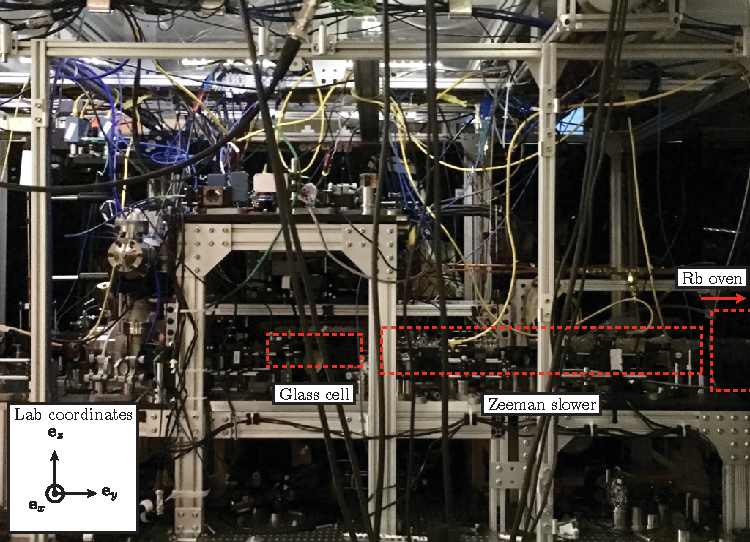
\includegraphics[]{Figures/Chapter4/RbLi_basic.pdf}
\caption[The RbLi vacuum system]{$\Rb87$ level structure (not to scale). {\bf a.} Ground and first excited state electronic configuration of $\Rb87$ given by the $\{n,\mathbf{L}\}$ quantum numbers. {\bf b.} The interaction between the orbital angular momentum and the spin of the electron leads to the fine splitting of orbitals with $L>0$. The splitting of the $5^2P$ line gives rise to the D1 and D2 lines. {\bf c.} The interaction between the total angular momentum and the nuclear spin causes the fine structure levels to split further into states characterized by the quantum number $F$.}
\label{fig:RbLi}
\end{center}
\end{figure*}

\subsection{Laser systems}

We use a total of three lasers to perform laser cooling of atoms: a cooling laser that addresses the $F=2\rightarrow F'=3$ transition, a repump laser that takes atoms that have decayed into the $F=1$ state back to $F=2$ and a master laser that provides a frequency reference for both lasers. The frequency of master laser is locked using saturation absorption spectroscopy to the $F=3\rightarrow F'=3$ and $F=3\rightarrow F'=4$ crossover of the D2 line of $^{85}$Rb.

We have to imaging systems. The first one is used primarily for diagnostics and it images the $yz$ plane of the atoms from the $+\ex$ side of the glass cell. The second system looks at the $xy$ plane from bellow the glass cell. 

\note{TODO:make basic sketch of lasers}

I discuss the Raman laser setup in Section~\ref{sec:Raman_laser}.

\section{Magnetic field control}

We use multiple coils to generate magnetic fields at the atoms. \note{TODO:make figure of coils}

One pair of anti-Helmholtz coils generates a strong quadrupole magnetic field along $\ez$ that is used in the making of the MOT and for magnetic trapping. Three pairs of Helmholtz coils in the vicinity of the glass cell generate bias magnetic fields along $\ex$, $\ey$ and $\ez$. The precise control of bias magnetic fields is essential during the multiple stages in our experimental sequence. Once BECs are produced we typically use bias fields along $\ez$ to change the Zeeman energy of the different $m_F$ states. An additional set of coils arranged in a `clover leaf' pattern generates small gradients along $\ez$, $\ex+\ey$ and $\ez-\ey$ which allow us to cancel stray magnetic gradients at the location of the atoms.  

The experiment has the capability of producing oscillatory magnetic fields. A set of coils on a printed circuit board produce linearly polarized RF magnetic fields either in the $\ey$ or $\ez$ direction that are used for RF induced evaporation and to drive transitions between $m_F$ states. 




\section{New master laser}
Previously we used a \noted{New Focus Vortex II TLB-6900} extended cavity diode laser as our master laser and a home made saturation spectroscopy setup using a Rb glass cell (see~\cite{CampbellThesis,PriceThesis}). The frequency of this laser was not very stable and the laser would constantly get out of lock. We replaced this laser with a \noted{Vescent photonics DBR Laser Moduee System} which uses a distributed Bragg reflector laser diode with no external cavity and is therefore very mechanically stable. The frequency of the laser is stabilized and controlled using the \noted{D2-210} spectroscopy module and \noted{D2-125} laser servo. The master laser system is considerably simplified as can be seen in Figure~\ref{fig:master_laser}.

\begin{figure*}[htb]
\begin{center}
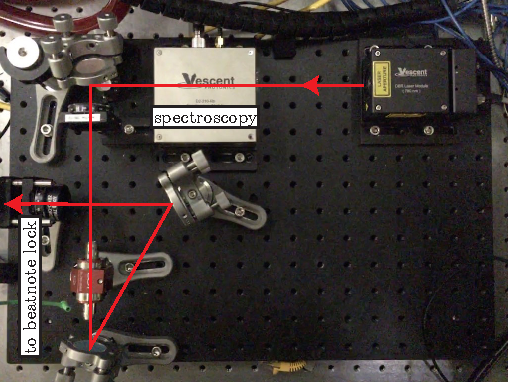
\includegraphics[]{Figures/Chapter4/master_laser.pdf}
\caption[Water cooling manifold schematic]{\note{TODO: write caption for plumbing figure.}}
\label{fig:master_laser}
\end{center}
\end{figure*}

\section{Small changes in MOT and imaging}

New Focus 8892-K motorized flipper mounts
-Flipper mirrors suck
-Polarimeter and PD for MOT diagnostics


\section{New Raman laser system}
\label{sec:Raman_laser}




\subsection{High power RF electronics}
\label{sec:high_power_rf_antenna}
The antenna loop is Digikey part number $732-5646-ND$

\subsection{$6.8$ GHz microwave electronics}

\section{Computer control and data acquisition}
Our lab has transitioned from using a \noted{LabVIEW} based control system to a Python based control system \noted{the labscriopt suite}. The new control software allows us to use scripted programming 

\noted{labscript} has 


his allowed us to use scripted programming on our devices
[161]. With labscript, a fuller exploration of the parameter spaces was feasible
and close-loop optimization of experimental parameters could be done online while
running the experiment.

\subsection{New xy camera}
-Mako camera is awesome


\section{Experimental sequence to make BECs}
\label{sec:making-becs}

\subsection{MOT}




-Trigger to the 60Hz line is essential. 

\subsection{Magnetic field stabilization with microwaves and partial transfer absorption imaging}
\label{sec:ptai}
We then apply a pair of $250\,\mu\mathrm{s}$ microwave  pulses that each transfer a small fraction of atoms into the $5^2{\rm S}_{1/2}$ $f=2$ manifold that we use to monitor and stabilize the bias field \cite{leblanc_direct_2013}. The microwave pulses are detuned by $\pm 2\, \kHz$ from the $\ket{f=1,m_F=0}\leftrightarrow\ket{f=2,m_F=1}$ transition and spaced in time by $33\, \mathrm{ms}$ (two periods of $60\, \mathrm{Hz}$). We imaged the transferred atoms following each pulse using absorption imaging\footnote{We did not apply repump light during this imaging, so the untransferred atoms in the $f=1$ manifold were largely undisturbed by the imaging process.}, and count the total number of atoms $n_1$ and $n_2$ transferred by each pulse. The imbalance in these atom numbers $(n_1-n_2)/(n_1+n_2)$ leads to a $4\kHz$ wide error signal that we use both to monitor the magnetic field before each spectroscopy measurement and cancel longterm drifts in the field. 

